\documentclass[11pt]{article}
\usepackage[margin=2.5cm]{geometry}
\usepackage{graphicx}
\usepackage{varwidth}
\usepackage{float}			%[H] for "exactly here"
\usepackage{amsfonts}		%Standard maths
\usepackage{amsmath}		%Standard maths
\usepackage{amssymb}		%Standard maths
\usepackage{caption}
\usepackage{listings}

\captionsetup[figure]{font=footnotesize}
\linespread{1.3}		%1.5 spacing
\lstset{language=Python,breaklines}		%,showtabs=true,tab=\rightarrowfill

\begin{document}

\thispagestyle{empty}
\title{UNIVERSITY OF READING\\
~\\
Department of Meteorology\\
~\\
On the Representation of Evaporation and Condensation in Weather Models}
\author{Jack Travis}
\maketitle

%declaration

\section{Abstract}
legue

\newpage

\tableofcontents

\newpage

\section{Problem}
\subsection{Description}
The main subject is to investigate how evaporation and condensation may behave under advection in a weather model. \\
Of interest are extreme cases, where a large amount of evaporation or condensation occurs over a short time/space interval, as in air being advected through a front. In such cases, models may predict more fluid undergoing evaporation or condensation than there is liquid or vapour available to evaporate or condense, leading to invalid values for fluid properties, possibly including instability. The primary subject is to examine and compare different methods of preventing adverse effects from occurring.\\
~\\
The example problem is of condensed fluid advecting over a region of high temperature, where evaporation is expected, and then returning to condensing. For the sake of example, the condensing/evaporating/condensing sections of the (one-dimensional) domain are taken to be equal thirds.

\subsection{Implementation}
The updating that occurs at each timestep $t$ is equivalent to the following for all $i\in\left[0,L/\Delta x\right]$:
\begin{align*}
	e^t_i &= \begin{cases}
		-Vapour^t_i / \frac{\Delta t}{2}		& : E_i > -Vapour^t_i / \frac{\Delta t}{2} \\
		Liquid^t_i / \frac{\Delta t}{2}		& : E_i > Liquid^t_i / \frac{\Delta t}{2} \\
		E_i & : \text{else}
	\end{cases} \\
	\begin{pmatrix}Vapour^{t+1/2}_i\\Liquid^{t+1/2}_i\end{pmatrix} &=
		\begin{pmatrix}Vapour^t_i\\Liquid^t_i\end{pmatrix}
		+ \frac{\Delta t}{2}\begin{pmatrix}e^t_i\\-e^t_i\end{pmatrix} \\
	\begin{pmatrix}\Delta Vapour^{t+1/2}_i\\\Delta Liquid^{t+1/2}_i\end{pmatrix} &= \begin{cases}
		\begin{pmatrix}Vapour^{t+1/2}_i - Vapour^{t+1/2}_{i-1}\\Liquid^{t+1/2}_i - Liquid^{t+1/2}_{i-1}\end{pmatrix}			& : i > 0 \\
		\begin{pmatrix}Vapour^{t+1/2}_i - Vapour^{t+1/2}_{\text{nice}}\\Liquid^{t+1/2}_i - Liquid^{t+1/2}_{\text{nice}}\end{pmatrix}	& : i = 0
	\end{cases} \\
	\begin{pmatrix}Vapour^{t+1}_i\\Liquid^{t+1}_i\end{pmatrix} &=
		\begin{pmatrix}Vapour^{t+1/2}_i\\Liquid^{t+1/2}_i\end{pmatrix}
		- \frac{u\Delta t}{2\Delta x}\begin{pmatrix}\Delta Vapour^{t+1/2}_i\\\Delta Liquid^{t+1/2}_i\end{pmatrix}
\end{align*}
Here $Vapour_{\text{nice}}$ and $Liquid_{\text{nice}}$ are the predefined ``nice'' values for the fluid's properties off the left edge of the domain, as the domain is taken to not wrap around.

\section{Development}
\subsection{Initial development, 30/4/18}
The problem was described in its basic form. Various details not described were decided upon in a sensible way. \\
~\\
The boundaries were treated as if fluid disappeared at the right edge of the domain and was spontaneously created at the left edge. The properties of the fluid coming in were assumed to be the same as the fluid upon the left edge at the initial timestep, taking this as a ``nice'' set of properties. Note that this only makes sense if $u$ is positive. In future, maybe incoming fluid varying over time could be used somehow.\\
The background velocity, $u$, was taken to be totally constant, fixed in time and space: varying velocity may be investigated, but it is of limited importance.\\
~\\
The model was designed handling $E$ (the evaporation/condensation rate) as unvarying in time but varying in space, and being sufficiently large as to completely evaporate or condensate all the moisture within 2 timesteps, i.e. being equal in magnitude to $1/(2\Delta t)$, since $\delta Vapour = E \delta t$. It is yet to be determined as to whether this is a sensible value.\\
In the example problem, $E$ is set to be equal to negative across the domain, except in the middle third of the domain where it is positive, with a hard step between these regions (sudden change between evaporation/condensation).\\
Initially, the model took $E$ to be 0 in the case that not enough liquid/vapour is present for the expected evaporation/condensation to occur. This is unrealistic, as evaporation/condensation would still be expected to occur to a lessened extent. Handling this properly is the next item expected to be worked on.\\
~\\
The units of the model were generally taken to be either dimensionless/dedimensionalised or irrelevant, e.g. the size of the domain was taken to be 1. It must be noted that currently the timestep is rather equal to 0.1, though this may be altered. Currently also a gridsize of 90 cells is being used, in order for it to be divisible by 3 (see initial conditions of $E$ above).\\
~\\
The model was implemented with an FTBS scheme. Since this was shown to produce large errors in advection at the evaporation/condensation interface, replacement with a scheme of a higher order of accuracy in space would be ideal.
Initial testing (following the model finishing basic development) showed that unsatisfactory errors will occur at the evaporation/condensation interface for sufficiently large values for the background velocity, large enough such that the Courant number exceeds roughly 0.8. Since the necessary values for $u$ are quite large anyway, we might not have to care much for this problem.\\
Initial testing was considered complete once the model produced more-or-less correct results for advection without evaporation/condensation (under initial conditions otherwise believed to be sensible) and vice versa. The model went through several iterations before this occurred.\\
~\\
Other than a potential switch to a better advection scheme, the next development should be to find how to correctly limit the evaporation/condensation such that no more fluid is evaporated/condensed per timestep than there is liquid/vapour available.

\subsection{3/5/18}
I investigated the errors that occur at the liquid/vapour interfaces and why they cause enormous oscillations for a large background velocity.\\
It turns out that the errors in FTBS that occur at the interfaces propagate across the domain by ordinary advection, decreasing in magnitude as they go. As a result, for a sufficiently large background velocity (roughly $u=0.0838$, $c=0.754$), it appears that the oscillations from the two interfaces overlap, resulting in a positive interference pattern. In addition, the errors seem to increase in magnitude with increasing background velocity anyway. \\
The effects, and how they change for increasing $u$, can be seen in figure \ref{fig:eighth} below.
\begin{figure}[H]
\centering
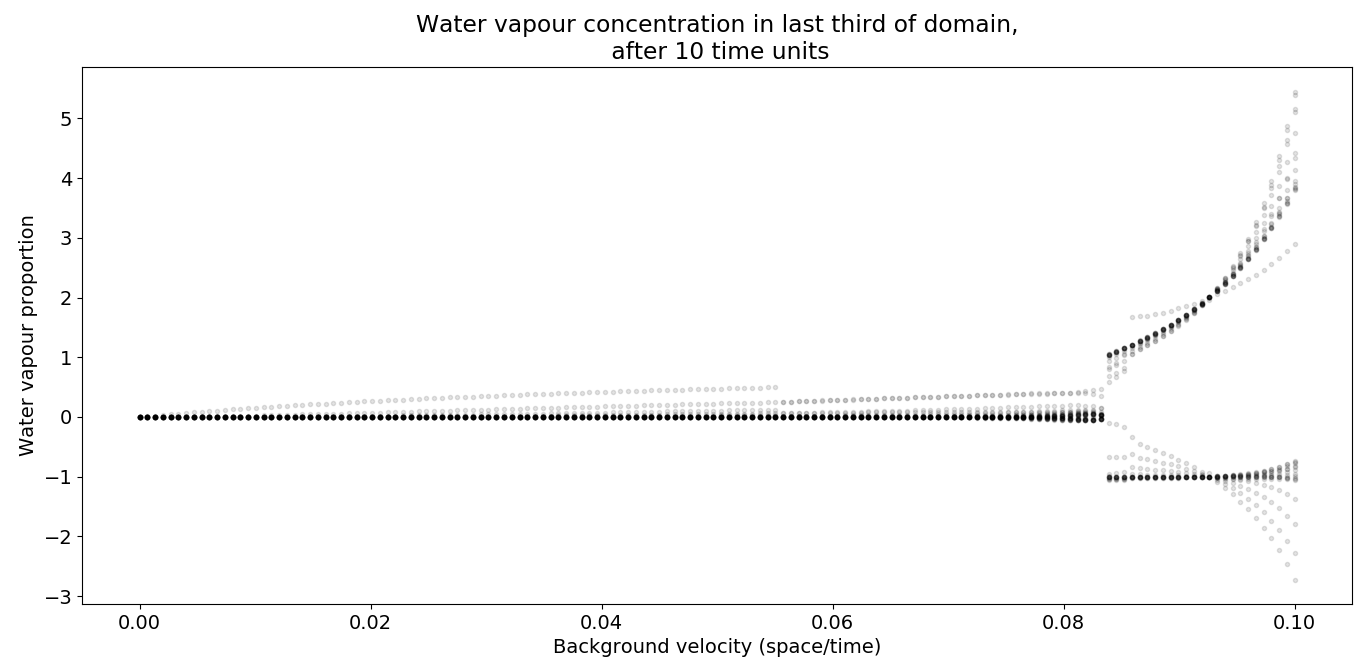
\includegraphics[width=\textwidth]{eighth}
\caption{A bifurcation diagram for the values of water vapour across the last third of the domain (a condensing region), after 10 arbitrary time units (with $\Delta t=0.1$, thus 100 timesteps), as varying with the background velocity. As $u$ increases, fluid from the middle third of the domain (an evaporating region) ``intrudes'' more and more upon the last third.}
\label{fig:eighth}
\end{figure}
\noindent I suspected, however, that this was due to an oversight in how the evaporation/condensation was limited, to ensure that no more liquid/vapour could evaporate/condense than there was liquid/vapour available. After realising the relevant section was incorrect, I replaced it with the following:
\begin{lstlisting}
#Evaporation = E
# if less liquid present than should be evaporated in one timestep:
if Liquid < E * Dt:
	# then Liquid should = E * Dt, thus
	E = Liquid / Dt
#Condensation = -E
# if less vapour present than should be condensed in one timestep:
if Vapour < -E * Dt:
	# then Vapour should = -E * Dt, thus
	E = -Vapour / Dt
\end{lstlisting}
However, using these limits did not produce significant differences in the system's behaviour. Thus, the problem is still not solved.

\subsection{12/5/18}
A certain reason for the failure of evaporation/condensation with a large background velocity was eventually found.\\
The two processes are calculated for at the same time. Hence, thinking of the two processes as totally separate, the evaporation/condensation that should affect a given portion of liquid/vapour is not actually applied to that part of the domain until after the liquid/vapour has advected away and different fluid has advected in. With the evaporation/condensation being calculated with reference to the old fluid values but applied to the new values, this can lead to the liquid/vapour values exiting their normal ranges (between 0 and 1). The FTBS advection of these invalid fluid values is the cause of the oscillating errors described previously.\\
The solution proposed is to separate the two processes such that evaporation/condensation occurs first, and then advection. Implementing this is the next important stage in development.\\
legue %discuss operator splitting based on paper

\subsection{17/5/18}
Operator splitting has been implemented: first evaporation/condensation occurs, then advection occurs separately. Each is considered its own time operation, thus using timesteps equal to $\Delta t/2$.\\
Interestingly, with the processes separated, the spacestep/timestep limits have been relaxed: relatively normal behaviour appears to be able to occur for Courant numbers greater than 1. The results can be seen in figures \ref{fig:eleventh} and \ref{fig:twelfth} below.
\begin{figure}[H]
\centering
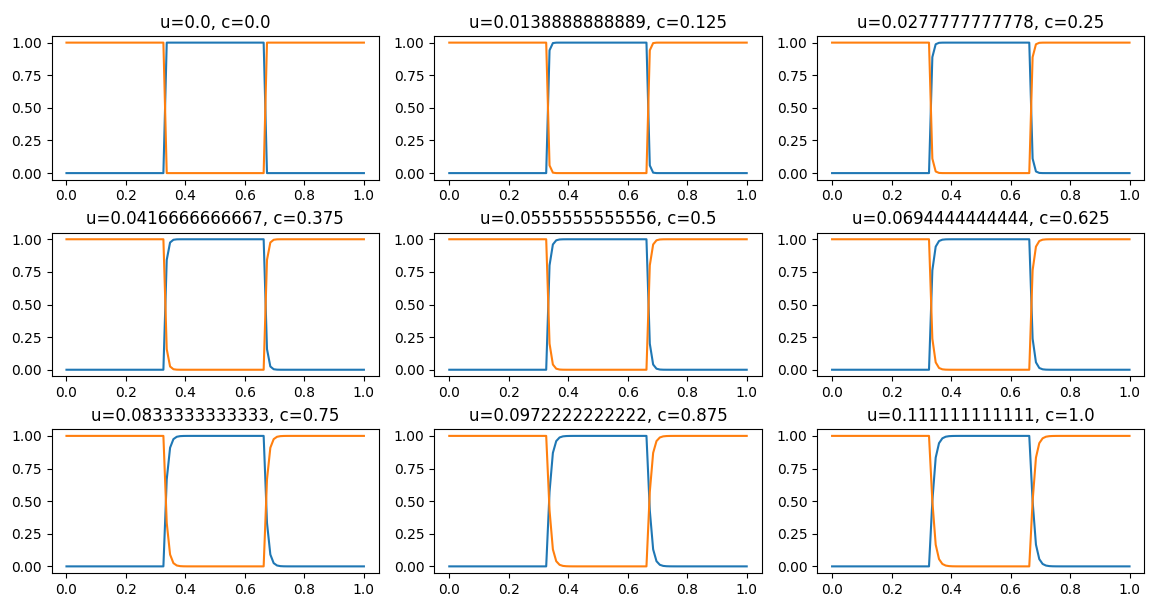
\includegraphics[width=\textwidth]{eleventh}
\caption{The fluid after 10 time units, for varying background velocities that give a Courant number less than 1.}
\label{fig:eleventh}
\end{figure}
\begin{figure}[H]
\centering
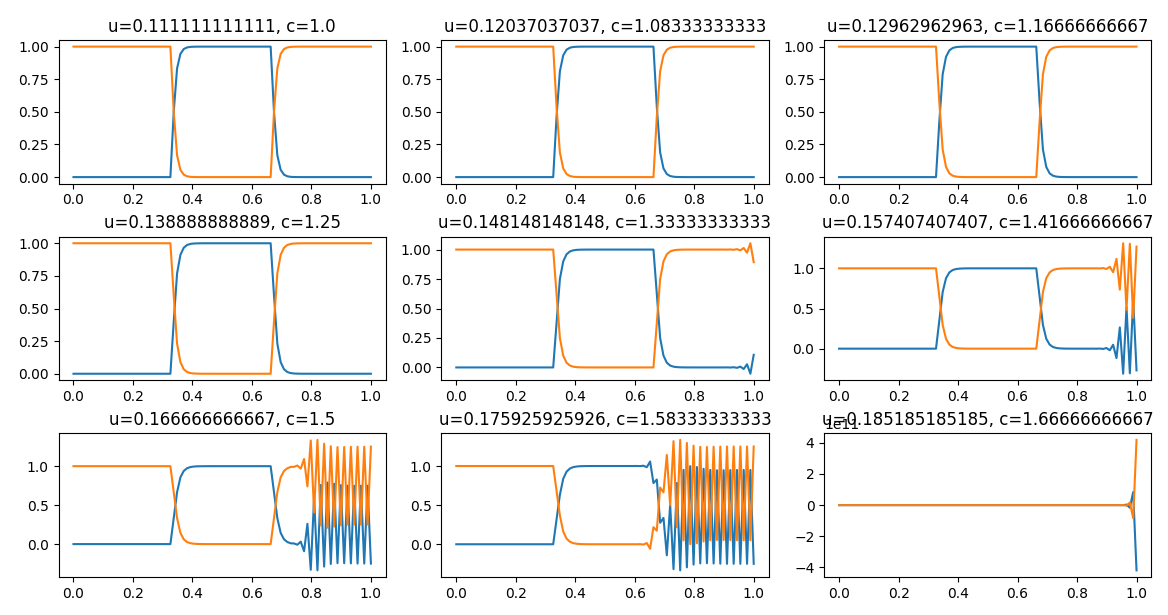
\includegraphics[width=\textwidth]{twelfth}
\caption{The fluid after 10 time units, for some background velocities that give a Courant number greater than 1.}
\label{fig:twelfth}
\end{figure}
\noindent The investigation of behaviour for Courant numbers greater than 1 may be the subject of further study. \\
~\\
The evaporation/condensation rate is currently a variable of its own, separate from anything else. The next step in development is to replace it with an evaporation/condensation function dependent on the vapour/liquid ratio, as well as upon temperature, which itself will have to become a variable of its own. \\
legue %discuss based on papers

\subsection{22/5/18}
It turned out that some of the behaviour in the previous simulation was due to a programming error. In particular, completely disregard figure \ref{fig:twelfth}, and instead understand behaviour for Courant numbers greater than 1 as follows in figure \ref{fig:thirteenth}.
\begin{figure}[H]
\centering
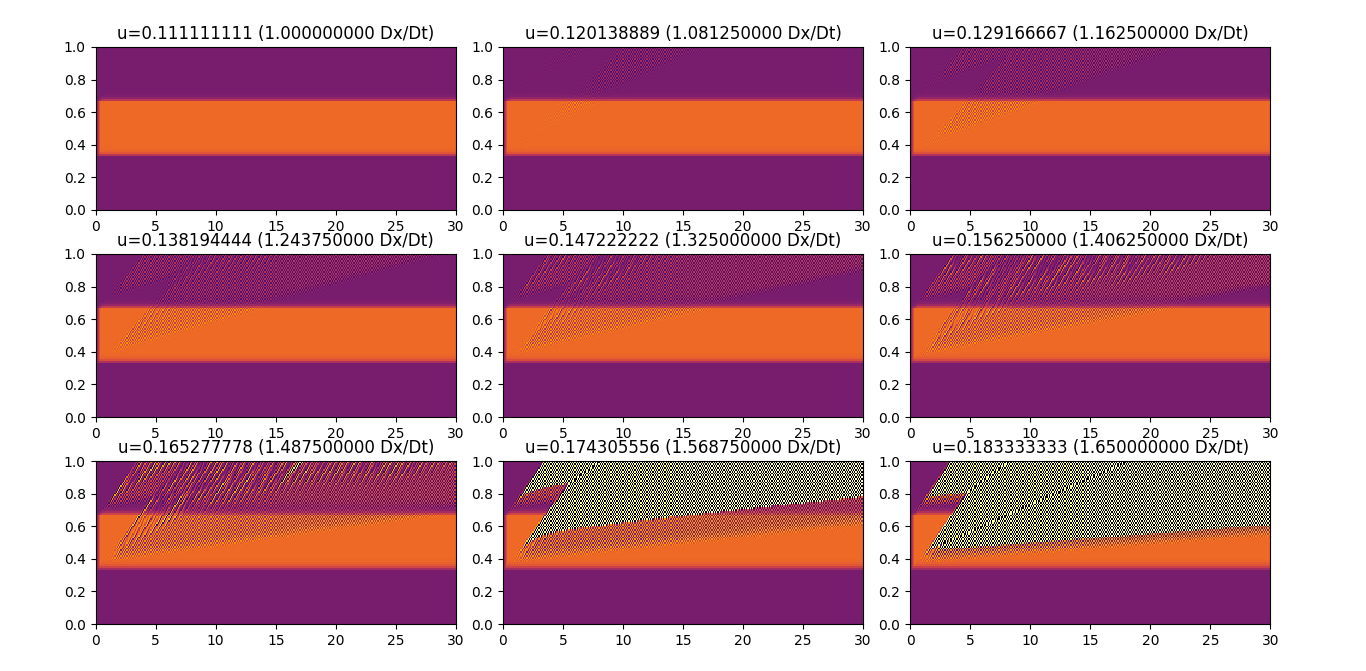
\includegraphics[width=\textwidth]{thirteenth}
\caption{The fluid over 30 time units, for some background velocities that give a Courant number greater than 1. Orange/white represents vapour, while purple/black represents liquid, with the white/black range being $Vapour=2$ to $Vapour=-1$. The solid black/white regions thus represent exploded oscillations.}
\label{fig:thirteenth}
\end{figure}
\noindent We find that for Courant numbers greater than 1, oscillatory errors occur. For Courant number slightly greater than 1, the errors form, grow to a certain extent, and are then eliminated by diffusion, with the rate at which they are eliminated being inversely proportional to the background velocity. This inverse proportionality means that for a sufficiently high background velocity, the diffusion is not enough to eliminate the errors, and they explode.
% mathematical basis?

\section{References}
legue
% B&F paper
% the two OS papers?

\end{document}